\chapter*{Introduction}
\markboth{\MakeUppercase{Introduction}}{\MakeUppercase{Introduction}}
\addcontentsline{toc}{chapter}{Introduction}

\improvement{Write introduction}

\begin{figure}
\centering
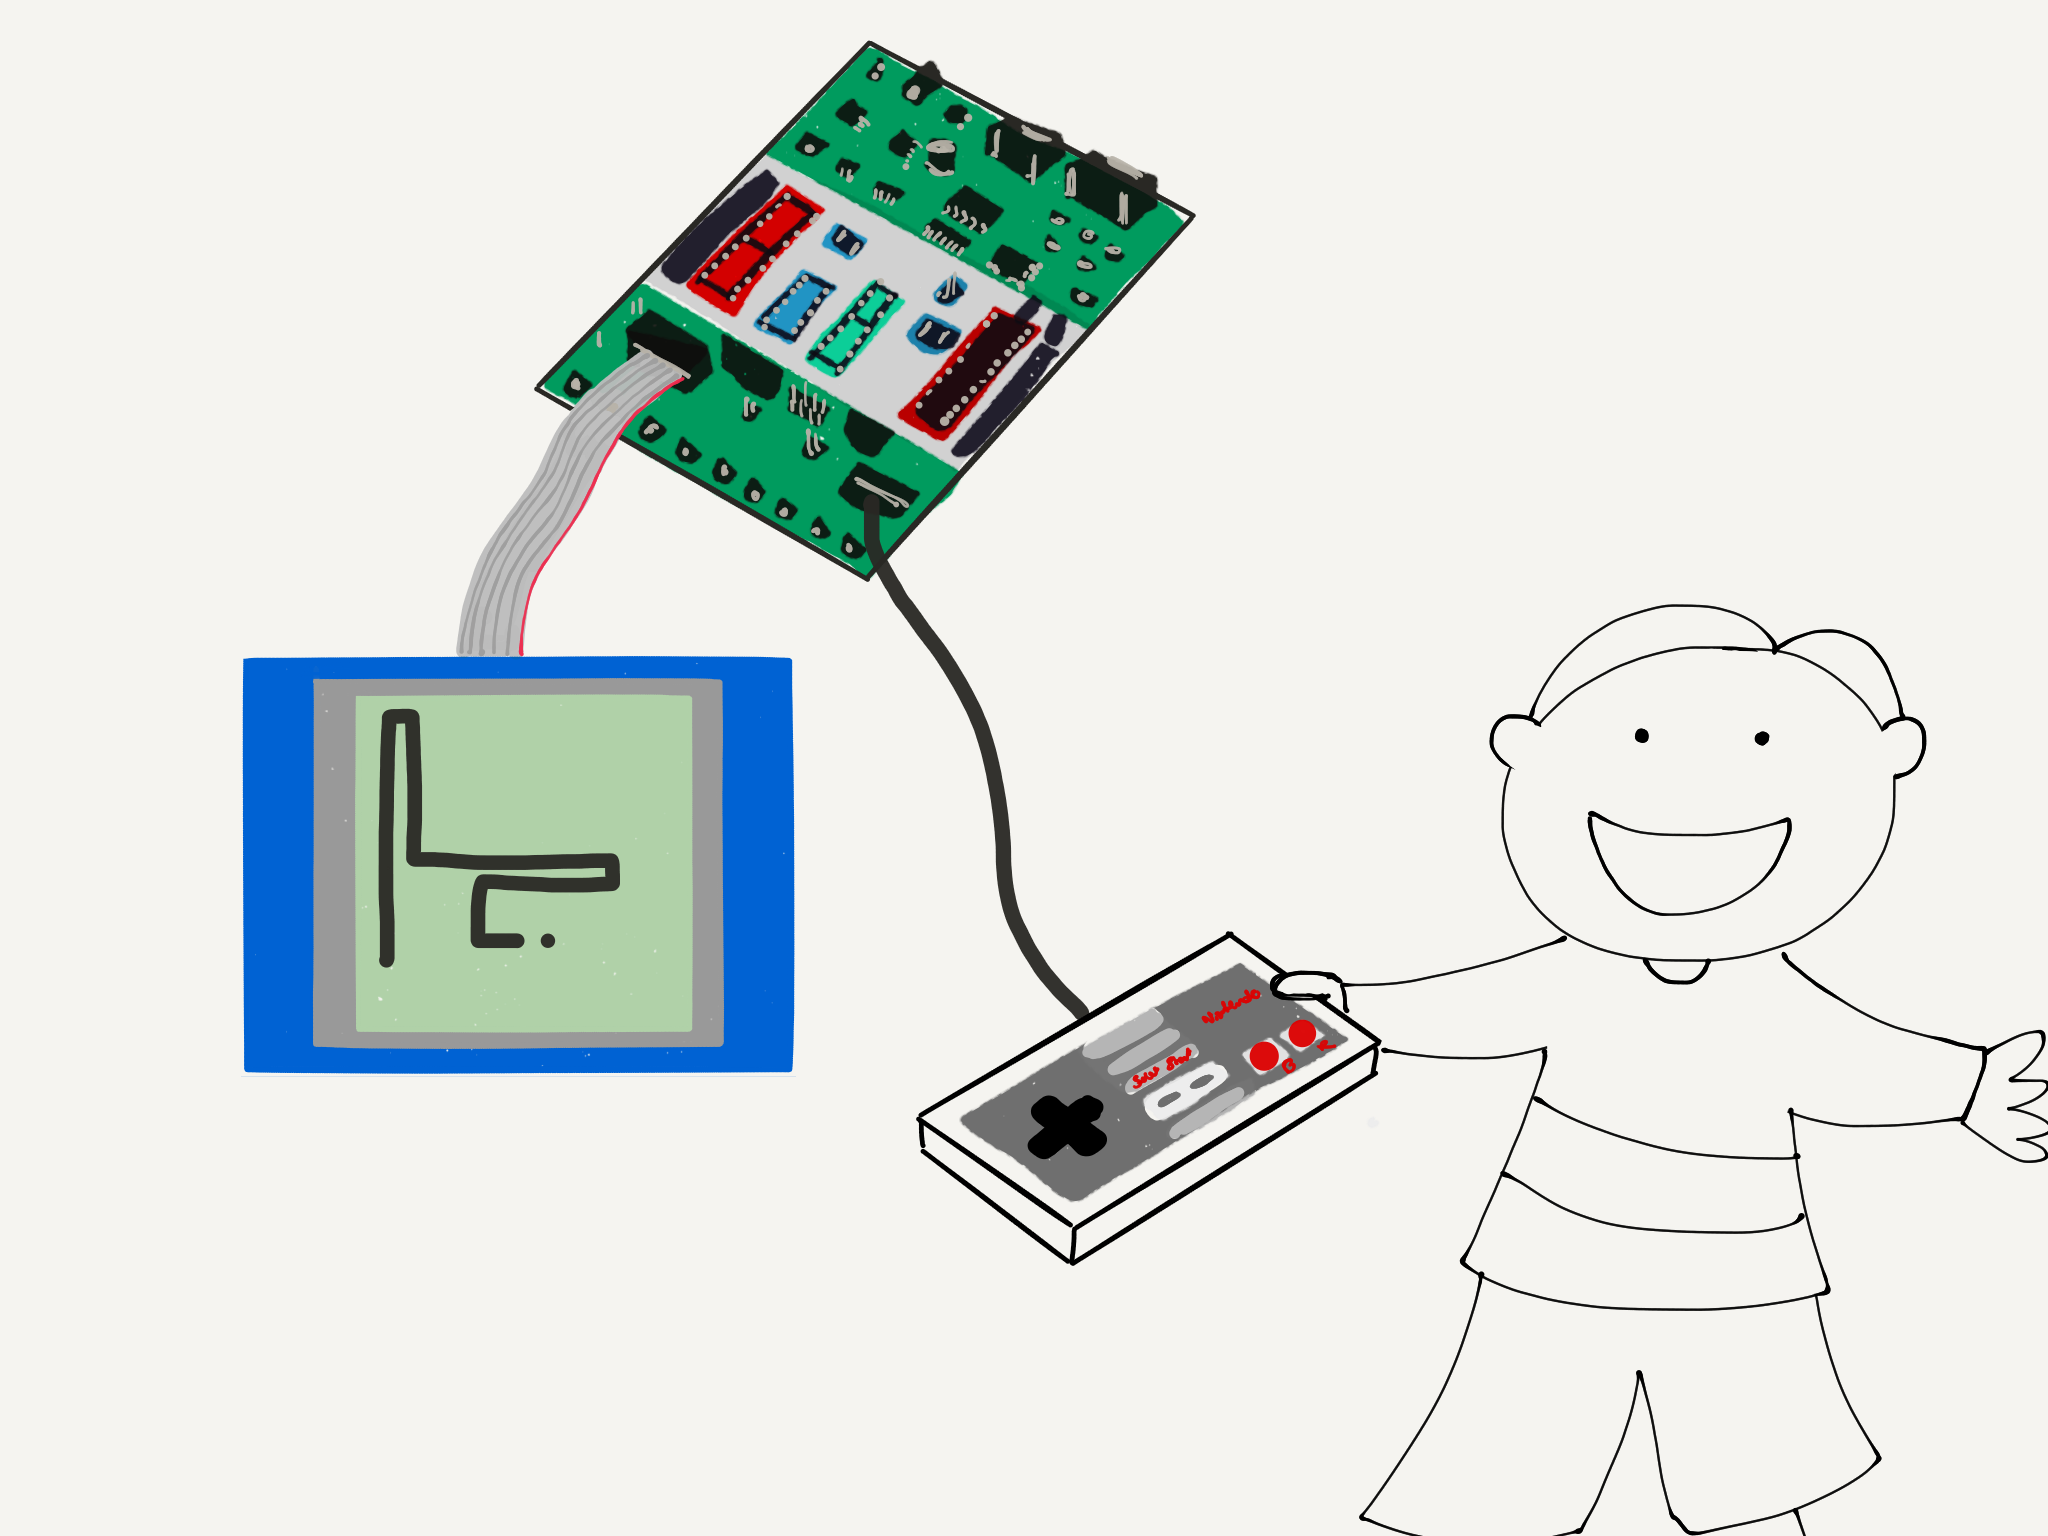
\includegraphics[width=.9\textwidth]{rigebillede.png}
\end{figure}

In this project we are trying to recreate the classic game snake as it was on the Nokia 3210 mobilephone.
We are doing this since we had access to a display from the nokia 3310 phone which is roughly the same display.

For this to work we need to write drivers for the microcontroller we are using in our case it will be an ATMEGA32 form Atmel.
We will try to write reusable drivers that could work with different mcu's of different clock frequencies and so on. 
These drivers are for interfaceing the display and the controller we are using. 

A large part of the project will be writing the main game code this will be done in C++ as opposed to C. 
We are doing this because we feel that C++ gives us certain advantages over C like having abstractions via classes.

The game logic for a snake game is actually quite simple all you have to do is check for collisons and then move the snake.
But that is just the snake part we need to have win/lose conditions and probably a pause menu. 

We also need to handle input and output, that means checking the controller for changes and then writing the new game state to the screen.
